% !TEX spellcheck = en_US

% ~~~~~~~~~~~~~~~~~~~~~~~~~~~~~~~~~~~~~~~ V
% (NC) 2026 Haluk Bingol
% github.com/halukbingol/LaTeX-Templates
%
% Licensees may copy, distribute, display, and perform the work and make derivative works
% and remixes based on it only for non-commercial purposes.
% ~~~~~~~~~~~~~~~~~~~~~~~~~~~~~~~~~~~~~~~ A

% v20261107T1230   user manual of hblibDatastructures.sty v20261104T2350
%
% hblibDatastructures-UserManual.tex -- every feature of hblibDatastructures.sty, as a deck:
% the LaTeX source next to the picture.
% Put it next to hblibPresentation.sty, hblibDatastructures.sty and hblibDataStructures.bib, then
%   pdflatex hblibDatastructures-UserManual
%   bibtex   hblibDatastructures-UserManual
%   pdflatex hblibDatastructures-UserManual
%   pdflatex hblibDatastructures-UserManual

\documentclass[aspectratio=169,10pt,compress]{beamer}




% ~~~~~~~~~~~~~~~~~~~~~~~~~~~~~~~~~~~~~~~~~~~~~~~~~~~~~~~~~~~~~~~~~ V hblib
	\usepackage{hblibPresentation}       % in a deck: \usepackage{../../hblib/hblibPresentation}
	\usepackage{hblibDatastructures}     % in a deck: \usepackage{../../hblib/hblibDatastructures}
% ~~~~~~~~~~~~~~~~~~~~~~~~~~~~~~~~~~~~~~~~~~~~~~~~~~~~~~~~~~~~~~~~~ A hblib




% +++++++++++++++++++++++++++++++++++++++ V specific
% texcode: LaTeX source in a light box (this manual only)
\lstdefinestyle{manualtex}{language={[LaTeX]TeX}, basicstyle=\ttfamily\scriptsize,
	frame=single, rulecolor=\color{gray!40}, backgroundcolor=\color{black!3},
	numbers=none, literate={}, columns=fullflexible, keepspaces=true, breaklines=true,
	showstringspaces=false, texcsstyle=*\color{blue!55!black}, commentstyle=\color{gray}\itshape,
	aboveskip=2pt, belowskip=2pt}
\lstnewenvironment{texcode}{\lstset{style=manualtex}}{}
% \swatch{color}: a small square of the color
\newcommand{\swatch}[1]{\textcolor{#1}{\rule{7pt}{7pt}}}
% +++++++++++++++++++++++++++++++++++++++ A specific




\title[hblibDatastructures: User Manual]{
	hblibDatastructures: User Manual
}
\subtitle{
	for hblibDatastructures.sty v20261104T2350
}
\author[Bingol]{Haluk Bingol}

\institute[FCIS]{
	Faculty of Computer and Information Sciences\\
	Yeditepe University
}
\date{{\tiny \hbTimeStamp}}

\begin{document}




% ~~~~~~~~~~~~~~~~~~~~~~~~~~~~~~~~~~~~~~ V frm
\begin{frame}[t,fragile]
	\titlepage
\end{frame}
% ~~~~~~~~~~~~~~~~~~~~~~~~~~~~~~~~~~~~~~ A frm




% ~~~~~~~~~~~~~~~~~~~~~~~~~~~~~~~~~~~~~~ V frm
\begin{frame}[t,fragile] \frametitle{Outline}
	\begin{columns}[T]
		\begin{column}{0.48\textwidth}
			\tableofcontents[sections={1-4}, hideallsubsections]
		\end{column}
		\begin{column}{0.48\textwidth}
			\tableofcontents[sections={5-8}, hideallsubsections]
		\end{column}
	\end{columns}
\end{frame}
% ~~~~~~~~~~~~~~~~~~~~~~~~~~~~~~~~~~~~~~ A frm




% ~~~~~~~~~~~~~~~~~~~~~~~~~~~~~~~~~~~~~~ V
\hSection[Start]{Getting started}{Loading, pictures, colors}
% ~~~~~~~~~~~~~~~~~~~~~~~~~~~~~~~~~~~~~~ A




% ~~~~~~~~~~~~~~~~~~~~~~~~~~~~~~~~~~~~~~ V frm
\begin{frame}[t,fragile] \frametitle{Loading and using the library}
	\begin{columns}[T]
		\begin{column}{0.52\textwidth}

% +++++++++++++++++++++++++++++++++++++++ V
%: -Code.
\begin{texcode}
\usepackage{../../hblib/hblibPresentation}
\usepackage{../../hblib/hblibDatastructures}

\begin{frame}[t,fragile] \frametitle{An array}
  \begin{center}
    \begin{tikzpicture}
      \hArray[name=a]{3,1,4,1,5}
    \end{tikzpicture}
  \end{center}
\end{texcode}
% +++++++++++++++++++++++++++++++++++++++ A

		\end{column}
		\begin{column}{0.44\textwidth}
			\begin{center}
				\begin{tikzpicture}
					\hArray[name=a]{3,1,4,1,5}
				\end{tikzpicture}
			\end{center}

			\begin{itemize}\footnotesize
				\item Every macro is used \hEmph{inside} a \hCode{tikzpicture}
				\item Lengths are in cm; the picture can have more nodes and arrows
				\item Load it after hblibPresentation; it also works in an article
			\end{itemize}
		\end{column}
	\end{columns}

% +++++++++++++++++++++++++++++++++++++++ V tbl
%: -Tbl. contents
\begin{table}
		\scriptsize
		\begin{tabular}{@{}L{0.20\textwidth}L{0.74\textwidth}@{}}
			\toprule
			\textbf{Draws} & \textbf{With} \\
			\midrule
			queue, stack & \hCode{\textbackslash hQueue}, \hCode{\textbackslash hStack} (array implementations as in CLRS~\cite{cormen2022introduction}) \\
			string, array, grid & \hCode{\textbackslash hString}, \hCode{\textbackslash hArray}, \hCode{\textbackslash hGrid}; styles \hCode{hvar}, \hCode{href} for references \\
			trees, commit graphs & TikZ styles \hCode{htree}, \hCode{hnode}, \dots; \hCode{hcommit}, \hCode{hbranch}, \dots \\
			\bottomrule
		\end{tabular}
\end{table}%
% +++++++++++++++++++++++++++++++++++++++ A tbl
\end{frame}
% ~~~~~~~~~~~~~~~~~~~~~~~~~~~~~~~~~~~~~~ A frm




% ~~~~~~~~~~~~~~~~~~~~~~~~~~~~~~~~~~~~~~ V frm
\begin{frame}[t,fragile] \frametitle{Colors}

% +++++++++++++++++++++++++++++++++++++++ V tbl
%: -Tbl. colors
\begin{table}
		\scriptsize
		\begin{tabular}{@{}L{0.24\textwidth}L{0.16\textwidth}L{0.52\textwidth}@{}}
			\toprule
			\textbf{Name} & \textbf{RGB} & \textbf{Used for} \\
			\midrule
			\swatch{colorTop} colorTop          & 55, 215, 0     & top of a stack; the current cell (\hCode{cur=}); \hCode{hhot} \\
			\swatch{colorTail} colorTail        & 55, 215, 0     & tail of a queue \\
			\swatch{colorHead} colorHead        & 255, 215, 0    & head of a queue; highlighted cells (\hCode{hot=}) \\
			\swatch{colorEmpty} colorEmpty      & 170, 255, 0    & an empty queue (head = tail) \\
			\swatch{colorUsed} colorUsed        & 238, 107, 110  & cells in use; \hCode{colorUsed!55}: visited (\hCode{done=}) \\
			\swatch{colorUnused} colorUnused    & 230, 230, 230  & cells not in use (\hCode{unused=}) \\
			\swatch{colorLabel} colorLabel      & 250, 118, 194  & the h and t marks of a queue \\
			\swatch{colorIndex} colorIndex      & 119, 118, 194  & index numbers; \hCode{href} arrows \\
			\swatch{colorBoxZero} colorBoxZero  & 160, 160, 160  & the unused cell 0 when indices start at 1 \\
			\bottomrule
		\end{tabular}
\end{table}%
% +++++++++++++++++++++++++++++++++++++++ A tbl

	\small Change one with \hCode{\textbackslash definecolor} after loading, e.g.\
	\hCode{\textbackslash definecolor\{colorHead\}\{RGB\}\{255,180,0\}}.
	colorIndex here (purple) replaces the blue colorIndex of hblibPresentation.
\end{frame}
% ~~~~~~~~~~~~~~~~~~~~~~~~~~~~~~~~~~~~~~ A frm




% ~~~~~~~~~~~~~~~~~~~~~~~~~~~~~~~~~~~~~~ V
\hSection[Queue, stack]{Queues and stacks}{\hCode{\textbackslash hQueue}, \hCode{\textbackslash hStack}}
% ~~~~~~~~~~~~~~~~~~~~~~~~~~~~~~~~~~~~~~ A




% ~~~~~~~~~~~~~~~~~~~~~~~~~~~~~~~~~~~~~~ V frm
\begin{frame}[t,fragile] \frametitle{\hCode{\textbackslash hQueue}: a circular queue in an array}

% +++++++++++++++++++++++++++++++++++++++ V
%: -Code.
\begin{texcode}
\hQueue{first}{capacity}{head}{tail}{e1,e2,...}[box width][box height]   % widths in cm: 0.8, 0.6
\end{texcode}
% +++++++++++++++++++++++++++++++++++++++ A

	\begin{itemize}\footnotesize
		\item \hCode{first}: 1 = indices 1 \dots\ capacity, cell 0 gray and not used (CLRS); 0 = indices 0 \dots\ capacity$-1$
		\item \hCode{head}: the first element (yellow, mark h); \hCode{tail}: the next free cell (green, mark t)
		\item In use: from head to tail$-1$, wrapping around (red); head = tail: empty (light green)
		\item The list fills the cells from the first index on; leave a place empty with nothing between commas
	\end{itemize}

	\begin{columns}[T]
		\begin{column}{0.48\textwidth}

% +++++++++++++++++++++++++++++++++++++++ V
%: -Code.
\begin{texcode}
\hQueue{1}{6}{2}{5}{,15,6,9}
\end{texcode}
% +++++++++++++++++++++++++++++++++++++++ A

			\begin{center}
				\begin{tikzpicture}
					\hQueue{1}{6}{2}{5}{,15,6,9}
				\end{tikzpicture}

				\footnotesize the queue 15, 6, 9; index 1 empty
			\end{center}
		\end{column}
		\begin{column}{0.48\textwidth}

% +++++++++++++++++++++++++++++++++++++++ V
%: -Code.
\begin{texcode}
\hQueue{1}{6}{5}{2}{3,,,,8,4}
\end{texcode}
% +++++++++++++++++++++++++++++++++++++++ A

			\begin{center}
				\begin{tikzpicture}
					\hQueue{1}{6}{5}{2}{3,,,,8,4}
				\end{tikzpicture}

				\footnotesize wrapped around: the queue 8, 4, 3
			\end{center}
		\end{column}
	\end{columns}
\end{frame}
% ~~~~~~~~~~~~~~~~~~~~~~~~~~~~~~~~~~~~~~ A frm




% ~~~~~~~~~~~~~~~~~~~~~~~~~~~~~~~~~~~~~~ V frm
\begin{frame}[t,fragile] \frametitle{\hCode{\textbackslash hQueue}: empty, first index 0, bigger boxes, step by step}
	\begin{columns}[T]
		\begin{column}{0.48\textwidth}

% +++++++++++++++++++++++++++++++++++++++ V
%: -Code.
\begin{texcode}
\hQueue{1}{6}{3}{3}{}               % empty
\hQueue{0}{6}{1}{4}{,5,7,2}         % indices 0..5
\hQueue{0}{4}{0}{2}{a,b}[1.0][0.7]  % bigger boxes
\end{texcode}
% +++++++++++++++++++++++++++++++++++++++ A

			\begin{center}
				\begin{tikzpicture} \hQueue{1}{6}{3}{3}{} \end{tikzpicture}\\[6pt]
				\begin{tikzpicture} \hQueue{0}{6}{1}{4}{,5,7,2} \end{tikzpicture}\\[6pt]
				\begin{tikzpicture} \hQueue{0}{4}{0}{2}{a,b}[1.0][0.7] \end{tikzpicture}
			\end{center}
		\end{column}
		\begin{column}{0.48\textwidth}

% +++++++++++++++++++++++++++++++++++++++ V
%: -Code.
\begin{texcode}
\only<1>{\hQueue{1}{5}{1}{1}{}}
\only<2>{\hQueue{1}{5}{1}{2}{7}}
\only<3>{\hQueue{1}{5}{1}{3}{7,2}}
\only<4>{\hQueue{1}{5}{2}{3}{,2}}
\end{texcode}
% +++++++++++++++++++++++++++++++++++++++ A

			\begin{center}
				\begin{tikzpicture}
					\only<1>{\hQueue{1}{5}{1}{1}{}}
					\only<2>{\hQueue{1}{5}{1}{2}{7}}
					\only<3>{\hQueue{1}{5}{1}{3}{7,2}}
					\only<4>{\hQueue{1}{5}{2}{3}{,2}}
				\end{tikzpicture}

				\footnotesize
				\only<1>{empty}\only<2>{enqueue 7}\only<3>{enqueue 2}\only<4>{dequeue: 7 leaves}
			\end{center}
		\end{column}
	\end{columns}
\end{frame}
% ~~~~~~~~~~~~~~~~~~~~~~~~~~~~~~~~~~~~~~ A frm




% ~~~~~~~~~~~~~~~~~~~~~~~~~~~~~~~~~~~~~~ V frm
\begin{frame}[t,fragile] \frametitle{\hCode{\textbackslash hStack}: a stack in an array}

% +++++++++++++++++++++++++++++++++++++++ V
%: -Code.
\begin{texcode}
\hStack{first}{capacity}{top}{e1,e2,...}[box width][box height]   % widths in cm: 0.5, 0.5
\end{texcode}
% +++++++++++++++++++++++++++++++++++++++ A

	\begin{itemize}\footnotesize
		\item \hCode{first} as in \hCode{\textbackslash hQueue}; \hCode{top}: the index of the top element (green, mark t)
		\item Below top: in use (red); above top: free (gray). Top below the first index: an empty stack
	\end{itemize}

	\begin{columns}[T]
		\begin{column}{0.48\textwidth}

% +++++++++++++++++++++++++++++++++++++++ V
%: -Code.
\begin{texcode}
\hStack{1}{6}{4}{15,6,2,9}
\hStack{0}{6}{2}{a,b,c}[0.7][0.6]
\end{texcode}
% +++++++++++++++++++++++++++++++++++++++ A

			\begin{center}
				\begin{tikzpicture} \hStack{1}{6}{4}{15,6,2,9} \end{tikzpicture}\\[6pt]
				\begin{tikzpicture} \hStack{0}{6}{2}{a,b,c}[0.7][0.6] \end{tikzpicture}
			\end{center}
		\end{column}
		\begin{column}{0.48\textwidth}

% +++++++++++++++++++++++++++++++++++++++ V
%: -Code.
\begin{texcode}
\only<1>{\hStack{1}{5}{2}{4,8}}
\only<2>{\hStack{1}{5}{3}{4,8,1}}  % push 1
\only<3>{\hStack{1}{5}{2}{4,8}}    % pop
\end{texcode}
% +++++++++++++++++++++++++++++++++++++++ A

			\begin{center}
				\begin{tikzpicture}
					\only<1>{\hStack{1}{5}{2}{4,8}}
					\only<2>{\hStack{1}{5}{3}{4,8,1}}
					\only<3>{\hStack{1}{5}{2}{4,8}}
				\end{tikzpicture}

				\footnotesize \only<1>{a stack 4, 8}\only<2>{push 1}\only<3>{pop: 1 leaves}
			\end{center}
		\end{column}
	\end{columns}
\end{frame}
% ~~~~~~~~~~~~~~~~~~~~~~~~~~~~~~~~~~~~~~ A frm




% ~~~~~~~~~~~~~~~~~~~~~~~~~~~~~~~~~~~~~~ V
\hSection[String, array]{Strings and arrays}{\hCode{\textbackslash hString}, \hCode{\textbackslash hArray}}
% ~~~~~~~~~~~~~~~~~~~~~~~~~~~~~~~~~~~~~~ A




% ~~~~~~~~~~~~~~~~~~~~~~~~~~~~~~~~~~~~~~ V frm
\begin{frame}[t,fragile] \frametitle{\hCode{\textbackslash hString}: characters and \hCode{substring}}

% +++++++++++++++++++++++++++++++++++++++ V
%: -Code.
\begin{texcode}
\hString[box width]{c,h,a,r,s}[from][to]        % box width 0.45 cm; boxes from <= i < to highlighted
\hString{H,e,l,l,o,\textvisiblespace,J,a,v,a}
\hString{H,e,l,l,o,\textvisiblespace,J,a,v,a}[1][4]   % s.substring(1, 4) is "ell"
\end{texcode}
% +++++++++++++++++++++++++++++++++++++++ A

	\begin{center}
		\begin{tikzpicture} \hString{H,e,l,l,o,\textvisiblespace,J,a,v,a} \end{tikzpicture}\\[10pt]
		\begin{tikzpicture} \hString{H,e,l,l,o,\textvisiblespace,J,a,v,a}[1][4] \end{tikzpicture}
	\end{center}

	\begin{itemize}\footnotesize
		\item One box per character, 0-based index above it
		\item \hCode{\textbackslash textvisiblespace} shows a space (\textvisiblespace); a comma must be given in braces: \hCode{\{,\}}
		\item The highlighted boxes are exactly the characters of \hCode{s.substring(from, to)}
	\end{itemize}
\end{frame}
% ~~~~~~~~~~~~~~~~~~~~~~~~~~~~~~~~~~~~~~ A frm




% ~~~~~~~~~~~~~~~~~~~~~~~~~~~~~~~~~~~~~~ V frm
\begin{frame}[t,fragile] \frametitle{\hCode{\textbackslash hArray[keys]\{e0,e1,\dots\}}: the keys}

% +++++++++++++++++++++++++++++++++++++++ V tbl
%: -Tbl. array keys
\begin{table}
		\scriptsize
		\begin{tabular}{@{}L{0.28\textwidth}L{0.20\textwidth}L{0.44\textwidth}@{}}
			\toprule
			\textbf{Key} & \textbf{Default} & \textbf{Meaning} \\
			\midrule
			\hCode{id=a}             & \hCode{hA}       & cell $i$ is the node \hCode{(a-i)}, e.g.\ \hCode{(a-0.west)} \\
			\hCode{at=\{(x,y)\}}     & \hCode{(0,0)}    & lower-left corner of cell 0 \\
			\hCode{width=}, \hCode{height=} & 0.6, 0.5 & box size in cm \\
			\hCode{name=scores}      & none             & a label on the left \\
			\hCode{index=}           & \hCode{above}    & \hCode{above}, \hCode{below} or \hCode{none} \\
			\hCode{hot=\{2\}}        & none             & highlighted cells (colorHead) \\
			\hCode{cur=\{3\}}        & none             & the current cell (colorTop) \\
			\hCode{done=\{0,1\}}     & none             & visited cells (colorUsed!55) \\
			\hCode{unused=\{5,...,7\}} & none           & cells not in use (colorUnused) \\
			\hCode{font=}            & \hCode{\textbackslash ttfamily\textbackslash small} & font of the elements \\
			\bottomrule
		\end{tabular}
\end{table}%
% +++++++++++++++++++++++++++++++++++++++ A tbl

	\small Lists use \hCode{\textbackslash foreach} syntax: \hCode{hot=\{0,...,3\}}.
	An element with a comma goes in braces: \hCode{\{\{1,2\},x\}}.
\end{frame}
% ~~~~~~~~~~~~~~~~~~~~~~~~~~~~~~~~~~~~~~ A frm




% ~~~~~~~~~~~~~~~~~~~~~~~~~~~~~~~~~~~~~~ V frm
\begin{frame}[t,fragile] \frametitle{\hCode{\textbackslash hArray}: keys in use}
	\begin{columns}[T]
		\begin{column}{0.55\textwidth}

% +++++++++++++++++++++++++++++++++++++++ V
%: -Code.
\begin{texcode}
\hArray{3,1,4,1,5}
\hArray[name=scores, index=below, width=0.8]{72,85,90,64}
\hArray[name=a, hot={1}, cur={3}, done={0}]{3,1,4,1,5}
\hArray[name=values, unused={4,...,7}, width=0.45, font=\ttfamily\scriptsize]{40,33,15,27,0,0,0,0}
\hArray[font=\ttfamily\scriptsize, width=0.9]{"ab",null,"c"}
\end{texcode}
% +++++++++++++++++++++++++++++++++++++++ A

		\end{column}
		\begin{column}{0.41\textwidth}
			\begin{tikzpicture}
				\hArray[at={(1.2,4.4)}]{3,1,4,1,5}
				\hArray[at={(1.2,3.2)}, name=scores, index=below, width=0.8]{72,85,90,64}
				\hArray[at={(1.2,1.9)}, name=a, hot={1}, cur={3}, done={0}]{3,1,4,1,5}
				\hArray[at={(1.2,0.8)}, name=values, unused={4,...,7}, width=0.45, font=\ttfamily\scriptsize]{40,33,15,27,0,0,0,0}
				\hArray[at={(1.2,-0.4)}, font=\ttfamily\scriptsize, width=0.9]{"ab",null,"c"}
			\end{tikzpicture}
		\end{column}
	\end{columns}

	\vspace{6pt}
	\small Several arrays in one picture: give each its own \hCode{at=\{(x,y)\}} (here they are stacked).
\end{frame}
% ~~~~~~~~~~~~~~~~~~~~~~~~~~~~~~~~~~~~~~ A frm




% ~~~~~~~~~~~~~~~~~~~~~~~~~~~~~~~~~~~~~~ V frm
\begin{frame}[t,fragile] \frametitle{\hCode{\textbackslash hArray}: node names, labels and reference arrows}
	\begin{columns}[T]
		\begin{column}{0.55\textwidth}

% +++++++++++++++++++++++++++++++++++++++ V
%: -Code.
\begin{texcode}
\hArray[id=r, at={(2.6,0)}, width=0.8, hot={0}]{99,2,3}
\node[hvar] (a) at (0.6,0.6) {};
\node[font=\ttfamily\small, left=2pt of a] {a};
\draw[href] (a.center) -- (r-0.west);
\node[hvar] (b) at (0.6,-0.4) {};
\node[font=\ttfamily\small, left=2pt of b] {b};
\draw[href] (b.center) -- (r-0.south west);
\node[colorIndex, font=\small] (ix) at (4.6,1.3) {index 2};
\draw[->, colorIndex] (ix) -- (r-2.north);
\end{texcode}
% +++++++++++++++++++++++++++++++++++++++ A

		\end{column}
		\begin{column}{0.41\textwidth}
			\begin{center}
				\begin{tikzpicture}
					\hArray[id=r, at={(2.6,0)}, width=0.8, hot={0}]{99,2,3}
					\node[hvar] (a) at (0.6,0.6) {};
					\node[font=\ttfamily\small, left=2pt of a] {a};
					\draw[href] (a.center) -- (r-0.west);
					\node[hvar] (b) at (0.6,-0.4) {};
					\node[font=\ttfamily\small, left=2pt of b] {b};
					\draw[href] (b.center) -- (r-0.south west);
					\node[colorIndex, font=\small] (ix) at (4.6,1.3) {index 2};
					\draw[->, colorIndex] (ix) -- (r-2.north);
				\end{tikzpicture}
			\end{center}

			\footnotesize
			\begin{itemize}
				\item \hCode{hvar}: a variable box; \hCode{href}: the arrow of a reference
				\item Two arrows to one array: \hCode{a} and \hCode{b} are aliases
				\item \hCode{left=2pt of a} needs TikZ's positioning library (hblibPresentation loads it)
			\end{itemize}
		\end{column}
	\end{columns}
\end{frame}
% ~~~~~~~~~~~~~~~~~~~~~~~~~~~~~~~~~~~~~~ A frm




% ~~~~~~~~~~~~~~~~~~~~~~~~~~~~~~~~~~~~~~ V frm
\begin{frame}[t,fragile] \frametitle{\hCode{\textbackslash hArray}: a loop, step by step}
	\begin{columns}[T]
		\begin{column}{0.55\textwidth}

% +++++++++++++++++++++++++++++++++++++++ V
%: -Code.
\begin{texcode}
\only<1>{\hArray[name=a, cur={0}]{72,85,90,64}}
\only<2>{\hArray[name=a, done={0}, cur={1}]{72,85,90,64}}
\only<3>{\hArray[name=a, done={0,1}, cur={2}]{72,85,90,64}}
\only<4>{\hArray[name=a, done={0,...,2}, cur={3}]{72,85,90,64}}
\only<5>{\hArray[name=a, done={0,...,3}]{72,85,90,64}}
\foreach \k in {0,...,4} {
  \only<\the\numexpr\k+1\relax>{%
    \node[font=\ttfamily\small] at (\k*0.6+0.3,-0.45) {i = \k};}
}
\end{texcode}
% +++++++++++++++++++++++++++++++++++++++ A

		\end{column}
		\begin{column}{0.41\textwidth}
			\begin{center}
				\begin{tikzpicture}
					\only<1>{\hArray[name=a, cur={0}]{72,85,90,64}}
					\only<2>{\hArray[name=a, done={0}, cur={1}]{72,85,90,64}}
					\only<3>{\hArray[name=a, done={0,1}, cur={2}]{72,85,90,64}}
					\only<4>{\hArray[name=a, done={0,...,2}, cur={3}]{72,85,90,64}}
					\only<5>{\hArray[name=a, done={0,...,3}]{72,85,90,64}}
					\foreach \k in {0,...,4} {
						\only<\the\numexpr\k+1\relax>{%
							\node[font=\ttfamily\small] at (\k*0.6+0.3,-0.45) {i = \k};}
					}
				\end{tikzpicture}
			\end{center}

			\footnotesize One \hCode{\textbackslash only} per slide; \hCode{cur} moves, \hCode{done} grows.
			The label follows \hCode{i}; at \hCode{i = 4} the loop stops.
		\end{column}
	\end{columns}
\end{frame}
% ~~~~~~~~~~~~~~~~~~~~~~~~~~~~~~~~~~~~~~ A frm




% ~~~~~~~~~~~~~~~~~~~~~~~~~~~~~~~~~~~~~~ V
\hSection[Grid]{Two-dimensional arrays}{\hCode{\textbackslash hGrid}}
% ~~~~~~~~~~~~~~~~~~~~~~~~~~~~~~~~~~~~~~ A




% ~~~~~~~~~~~~~~~~~~~~~~~~~~~~~~~~~~~~~~ V frm
\begin{frame}[t,fragile] \frametitle{\hCode{\textbackslash hGrid[keys]\{\{row 0\},\{row 1\},\dots\}}}

% +++++++++++++++++++++++++++++++++++++++ V
%: -Code.
\begin{texcode}
\hGrid[name=t]{{1,2,3},{4,5,6}}                                    % a 2 x 3 table
\hGrid[name=r, index=rows]{{7},{8,9},{1,2,3}}                      % ragged: rows of different lengths
\hGrid[name=m, rowhot={1}, colhot={2}, cur={1/2}]{{1,2,3},{4,5,6},{7,8,9}}
\end{texcode}
% +++++++++++++++++++++++++++++++++++++++ A

	\begin{columns}[T]
		\begin{column}{0.30\textwidth}
			\begin{center}
				\begin{tikzpicture} \hGrid[name=t]{{1,2,3},{4,5,6}} \end{tikzpicture}
			\end{center}
		\end{column}
		\begin{column}{0.30\textwidth}
			\begin{center}
				\begin{tikzpicture} \hGrid[name=r, index=rows]{{7},{8,9},{1,2,3}} \end{tikzpicture}
			\end{center}
		\end{column}
		\begin{column}{0.30\textwidth}
			\begin{center}
				\begin{tikzpicture} \hGrid[name=m, rowhot={1}, colhot={2}, cur={1/2}]{{1,2,3},{4,5,6},{7,8,9}} \end{tikzpicture}
			\end{center}
		\end{column}
	\end{columns}

	\begin{itemize}\footnotesize
		\item One brace group per row, row 0 on top; cell \hCode{(r,c)} is the node \hCode{(<id>-r-c)}, e.g.\ \hCode{(g-1-2.east)}
		\item Keys as in \hCode{\textbackslash hArray} (\hCode{id}, \hCode{at}, \hCode{width}, \hCode{height}, \hCode{name}, \hCode{font});
		cells are given as \hCode{r/c}: \hCode{hot=\{1/2,0/0\}}, \hCode{cur}, \hCode{done}, \hCode{unused}
		\item \hCode{rowhot=\{1\}}, \hCode{colhot=\{2\}}: whole rows, whole columns;
		\hCode{index=} \hCode{both} (default), \hCode{rows}, \hCode{cols} or \hCode{none}
	\end{itemize}
\end{frame}
% ~~~~~~~~~~~~~~~~~~~~~~~~~~~~~~~~~~~~~~ A frm




% ~~~~~~~~~~~~~~~~~~~~~~~~~~~~~~~~~~~~~~ V frm
\begin{frame}[t,fragile] \frametitle{\hCode{\textbackslash hGrid}: an array of rows}
	\begin{columns}[T]
		\begin{column}{0.55\textwidth}

% +++++++++++++++++++++++++++++++++++++++ V
%: -Code.
\begin{texcode}
\hGrid[id=g, at={(1.6,0)}, hot={1/2}]{{1,2,3},{4,5,6}}
\node[hvar] (t) at (0,0.25) {};
\node[font=\ttfamily\small, left=2pt of t] {t};
\draw[href] (t.center) -- (g-0-0.west);
\node[font=\small, colorIndex] (c) at (4.0,1.3) {\hCode{t[1][2]}};
\draw[->, colorIndex] (c) -- (g-1-2.north east);
\end{texcode}
% +++++++++++++++++++++++++++++++++++++++ A

		\end{column}
		\begin{column}{0.41\textwidth}
			\begin{center}
				\begin{tikzpicture}
					\hGrid[id=g, at={(1.6,0)}, hot={1/2}]{{1,2,3},{4,5,6}}
					\node[hvar] (t) at (0,0.25) {};
					\node[font=\ttfamily\small, left=2pt of t] {t};
					\draw[href] (t.center) -- (g-0-0.west);
					\node[font=\small, colorIndex] (c) at (4.0,1.3) {\hCode{t[1][2]}};
					\draw[->, colorIndex] (c) -- (g-1-2.north east);
				\end{tikzpicture}
			\end{center}

			\footnotesize Row $r$ is drawn $r \times$ height lower than row 0;
			the cell nodes make arrows and labels easy.
		\end{column}
	\end{columns}
\end{frame}
% ~~~~~~~~~~~~~~~~~~~~~~~~~~~~~~~~~~~~~~ A frm




% ~~~~~~~~~~~~~~~~~~~~~~~~~~~~~~~~~~~~~~ V
\hSection[Trees]{Trees}{Styles htree, hnode, hhot, hdone, hleaf, horder, hsquare}
% ~~~~~~~~~~~~~~~~~~~~~~~~~~~~~~~~~~~~~~ A




% ~~~~~~~~~~~~~~~~~~~~~~~~~~~~~~~~~~~~~~ V frm
\begin{frame}[t,fragile] \frametitle{A tree with TikZ's \hCode{child} syntax}
	\begin{columns}[T]
		\begin{column}{0.55\textwidth}

% +++++++++++++++++++++++++++++++++++++++ V
%: -Code.
\begin{texcode}
\begin{tikzpicture}[htree,
    level 1/.style={sibling distance=2.4cm},
    level 2/.style={sibling distance=1.2cm}]
  \node[hnode, hdone, horder=1] {8}
    child {node[hnode, hdone, horder=2] {3}
      child {node[hnode, hleaf] {1}}
      child {node[hnode, hleaf] {6}}}
    child {node[hnode, hhot, horder=3] {10}
      child[missing]
      child {node[hnode, hleaf] {14}}};
\end{tikzpicture}
\end{texcode}
% +++++++++++++++++++++++++++++++++++++++ A

		\end{column}
		\begin{column}{0.41\textwidth}
			\begin{center}
				\begin{tikzpicture}[htree,
						level 1/.style={sibling distance=2.4cm},
						level 2/.style={sibling distance=1.2cm}]
					\node[hnode, hdone, horder=1] {8}
						child {node[hnode, hdone, horder=2] {3}
							child {node[hnode, hleaf] {1}}
							child {node[hnode, hleaf] {6}}}
						child {node[hnode, hhot, horder=3] {10}
							child[missing]
							child {node[hnode, hleaf] {14}}};
				\end{tikzpicture}
			\end{center}

			\footnotesize
			\begin{itemize}
				\item \hCode{htree}: level distance, gray edges; \hCode{hnode}: a round node
				\item \hCode{hhot}: current; \hCode{hdone}: visited; \hCode{hleaf}: a leaf
				\item \hCode{horder=k}: the visit number $k$; \hCode{child[missing]}: an empty place
			\end{itemize}
		\end{column}
	\end{columns}
\end{frame}
% ~~~~~~~~~~~~~~~~~~~~~~~~~~~~~~~~~~~~~~ A frm




% ~~~~~~~~~~~~~~~~~~~~~~~~~~~~~~~~~~~~~~ V frm
\begin{frame}[t,fragile] \frametitle{\hCode{hsquare}: an expression tree}
	\begin{columns}[T]
		\begin{column}{0.55\textwidth}

% +++++++++++++++++++++++++++++++++++++++ V
%: -Code.
\begin{texcode}
\begin{tikzpicture}[htree, level 1/.style={sibling distance=2cm},
    level 2/.style={sibling distance=1.1cm}]
  \node[hsquare] {$*$}
    child {node[hsquare] {$+$}
      child {node[hnode] {2}}
      child {node[hnode] {3}}}
    child {node[hnode] {4}};
\end{tikzpicture}
\end{texcode}
% +++++++++++++++++++++++++++++++++++++++ A

		\end{column}
		\begin{column}{0.41\textwidth}
			\begin{center}
				\begin{tikzpicture}[htree, level 1/.style={sibling distance=2cm},
						level 2/.style={sibling distance=1.1cm}]
					\node[hsquare] {$*$}
						child {node[hsquare] {$+$}
							child {node[hnode] {2}}
							child {node[hnode] {3}}}
						child {node[hnode] {4}};
				\end{tikzpicture}
			\end{center}

			\footnotesize $(2 + 3) * 4$: operators in squares, numbers in circles.
			\hCode{hsquare} also suits folders.
		\end{column}
	\end{columns}
\end{frame}
% ~~~~~~~~~~~~~~~~~~~~~~~~~~~~~~~~~~~~~~ A frm




% ~~~~~~~~~~~~~~~~~~~~~~~~~~~~~~~~~~~~~~ V
\hSection[Commits]{Commit graphs}{Styles hcommit, hbranch, hheadref, htag, hparent}
% ~~~~~~~~~~~~~~~~~~~~~~~~~~~~~~~~~~~~~~ A




% ~~~~~~~~~~~~~~~~~~~~~~~~~~~~~~~~~~~~~~ V frm
\begin{frame}[t,fragile] \frametitle{A commit graph (version control)}
	\begin{columns}[T]
		\begin{column}{0.55\textwidth}

% +++++++++++++++++++++++++++++++++++++++ V
%: -Code.
\begin{texcode}
\node[hcommit] (c1) at (0,0)     {a1f};
\node[hcommit] (c2) at (1.3,0)   {b27};
\node[hcommit, hhot] (c3) at (2.6,0) {c3e};
\node[hcommit] (f1) at (2.6,-1.2) {d4a};
\draw[hparent] (c2) -- (c1);
\draw[hparent] (c3) -- (c2);
\draw[hparent] (f1) -- (c2);
\node[hbranch, above=3pt of c3] (m) {main};
\node[hheadref, above=2pt of m] {HEAD};
\node[hbranch, right=4pt of f1] {feature};
\node[htag, above=3pt of c1] {v1.0};
\end{texcode}
% +++++++++++++++++++++++++++++++++++++++ A

		\end{column}
		\begin{column}{0.41\textwidth}
			\begin{center}
				\begin{tikzpicture}
					\node[hcommit] (c1) at (0,0)     {a1f};
					\node[hcommit] (c2) at (1.3,0)   {b27};
					\node[hcommit, hhot] (c3) at (2.6,0) {c3e};
					\node[hcommit] (f1) at (2.6,-1.2) {d4a};
					\draw[hparent] (c2) -- (c1);
					\draw[hparent] (c3) -- (c2);
					\draw[hparent] (f1) -- (c2);
					\node[hbranch, above=3pt of c3] (m) {main};
					\node[hheadref, above=2pt of m] {HEAD};
					\node[hbranch, right=4pt of f1] {feature};
					\node[htag, above=3pt of c1] {v1.0};
				\end{tikzpicture}
			\end{center}

			\footnotesize
			\begin{itemize}
				\item An arrow points from a commit to its \hEmph{parent}
				\item \hCode{hbranch}: a branch name; \hCode{hheadref}: HEAD; \hCode{htag}: a tag
				\item \hCode{hhot}, \hCode{hdone} color a commit, as in trees
			\end{itemize}
		\end{column}
	\end{columns}
\end{frame}
% ~~~~~~~~~~~~~~~~~~~~~~~~~~~~~~~~~~~~~~ A frm




% ~~~~~~~~~~~~~~~~~~~~~~~~~~~~~~~~~~~~~~ V
\hSection[Notes]{Notes and troubleshooting}
% ~~~~~~~~~~~~~~~~~~~~~~~~~~~~~~~~~~~~~~ A




% ~~~~~~~~~~~~~~~~~~~~~~~~~~~~~~~~~~~~~~ V frm
\begin{frame}[t,fragile] \frametitle{Troubleshooting}

% +++++++++++++++++++++++++++++++++++++++ V tbl
%: -Tbl. troubleshooting
\begin{table}
		\scriptsize
		\begin{tabular}{@{}L{0.36\textwidth}L{0.28\textwidth}L{0.28\textwidth}@{}}
			\toprule
			\textbf{Message or problem} & \textbf{Cause} & \textbf{Fix} \\
			\midrule
			Missing \textbackslash begin\{document\}, or nodes in odd places & a macro outside a \hCode{tikzpicture} & put it inside one \\
			two arrays drawn on top of each other & both start at (0,0) & \hCode{at=\{(x,y)\}} \\
			``No shape named a-3'' & wrong \hCode{id}, or a cell that does not exist & \hCode{id=a}; cells are 0 \dots\ $n-1$ \\
			an element splits in two & a comma in the element & braces: \hCode{\{1,2\}} \\
			\hCode{\textbackslash hQueue} elements in the wrong cells & the list starts at the first index & leave cells empty: \hCode{\{,15,6\}} \\
			``I do not know the key \dots'' & a misspelled key of \hCode{\textbackslash hArray} & see the keys table \\
			``... of a'' does not work & positioning library not loaded & load hblibPresentation, or \hCode{\textbackslash usetikzlibrary\{positioning\}} \\
			indices purple, not blue & this library's colorIndex & \hCode{\textbackslash definecolor\{colorIndex\}\{\dots\}} \\
			\bottomrule
		\end{tabular}
\end{table}%
% +++++++++++++++++++++++++++++++++++++++ A tbl
\end{frame}
% ~~~~~~~~~~~~~~~~~~~~~~~~~~~~~~~~~~~~~~ A frm




% ~~~~~~~~~~~~~~~~~~~~~~~~~~~~~~~~~~~~~~ V frm
\begin{frame}[t,fragile] \frametitle{Quick reference}

% +++++++++++++++++++++++++++++++++++++++ V tbl
%: -Tbl. quick reference
\begin{table}
		\scriptsize
		\begin{tabular}{@{}L{0.55\textwidth}L{0.37\textwidth}@{}}
			\toprule
			\textbf{Command or style} & \textbf{Draws} \\
			\midrule
			\hCode{\textbackslash hQueue\{first\}\{capacity\}\{head\}\{tail\}\{e1,...\}[w][h]} & a circular queue \\
			\hCode{\textbackslash hStack\{first\}\{capacity\}\{top\}\{e1,...\}[w][h]} & a stack \\
			\hCode{\textbackslash hString[w]\{c,h,a,r,s\}[from][to]} & a string, substring highlighted \\
			\hCode{\textbackslash hArray[keys]\{e0,e1,...\}} & an array; nodes \hCode{(id-i)} \\
			\hCode{\textbackslash hGrid[keys]\{\{row 0\},\{row 1\},...\}} & a 2D array; nodes \hCode{(id-r-c)} \\
			\hCode{hvar}, \hCode{href} & a reference variable and its arrow \\
			\hCode{htree}, \hCode{hnode}, \hCode{hsquare}, \hCode{hhot}, \hCode{hdone}, \hCode{hleaf}, \hCode{horder=k} & trees \\
			\hCode{hcommit}, \hCode{hbranch}, \hCode{hheadref}, \hCode{htag}, \hCode{hparent} & commit graphs \\
			\bottomrule
		\end{tabular}
\end{table}%
% +++++++++++++++++++++++++++++++++++++++ A tbl
\end{frame}
% ~~~~~~~~~~~~~~~~~~~~~~~~~~~~~~~~~~~~~~ A frm




% ~~~~~~~~~~~~~~~~~~~~~~~~~~~~~~~~~~~~~~ V frm
\begin{frame}[t,fragile] \frametitle{References}
	\setbeamertemplate{bibliography item}[text]
	\bibliographystyle{IEEEtran}
	\tiny\bibliography{hblibDataStructures}
\end{frame}
% ~~~~~~~~~~~~~~~~~~~~~~~~~~~~~~~~~~~~~~ A frm



\end{document}
